%-----------------------------------------------------------------------------%
\chapter{IMPLEMENTASI DAN PENGUJIAN}
%-----------------------------------------------------------------------------%

\vspace{4.5pt}

\section{Lingkungan Implementasi}
Pada bagian ini dijelaskan mengenai spesifikasi perangkat keras dan kondisi lingkungan perangkat lunak yang digunakan selama proses implementasi dekomposisi dan pengujian.\\

\subsection{Spesifikasi Perangkat Keras}
Berikut spesifikasi perangkat keras untuk proses implementasi dekomposisi:

\begin{enumerate}[leftmargin=1.3cm]
	\item Nama Produk : Macbook Air 2020 
	\item Processor : Apple M1 8 Core CPU
	\item Memori : 8 GB
	\item Penyimpanan : 256 GB 
\end{enumerate}
Detail Spesifikasi perangkat keras di \textit{virtual machine}: 

\begingroup
\setlength{\LTleft}{-20cm plus -1fill}
\setlength{\LTright}{\LTleft}
\begin{small}
	\begin{longtable}{|p{6.5cm}|p{3cm}|p{3cm}|}
		\caption{Tabel Spesifikasi berserta aplikasi yang dijalankan di Virtual Machine}\\
		\hline
		\textbf{Virtual Machine} & \textbf{CPU} & \textbf{Memory}\\
		\endfirsthead

		\hline
		Odoo Monolith &  \multirow{2}{*}{2 Core}  & \multirow{2}{*}{2 GB} \\
		\cline{1-1}
		 	PostgreSQL &  & \\
		\hline
		Odoo Monolith &  \multirow{5}{*}{2 Core}  & \multirow{5}{*}{2 GB} \\
		\cline{1-1}
		 	PostgreSQL &  & \\
		\cline{1-1}
			Kong Gateway &  &\\
		\cline{1-1}
			Point of Sale Service &  &\\
		\cline{1-1}
			Product Service &  &\\
		\cline{1-1}
			MariaDB &  &\\
		\hline
	\end{longtable}
\end{small}
\endgroup

\subsection{Lingkungan Perangkat Lunak}
Berikut lingkungan perangkat lunak:

\begin{enumerate}[leftmargin=1.3cm]
	\item Sistem Operasi: macOS Ventura
	\item IDE : Visual Studio Code, GoLand 
	\item Tools : Dbeaver, Postman, Docker, Primate
	\item Bahasa Pemrograman: Python 3.8.2rc2, Go v1.20.4
\end{enumerate}

\section{Implementasi Perangkat Lunak}
Pada bagian ini dijelaskan bagaimana proses dekomposisi menggunakan Hierarchical Clustering dan dekomposisi aplikasi monolith menjadi microservice.

\subsection{\textit{Proses Clustering}}
Pada sub bab ini akan menjelaskan mengenai proses, fungsi, dan metode yang digunakan dalam proses clustering untuk menemukan kelompok service di aplikasi monolitik yaitu Odoo. \\

\subsubsection{Pengambilan Source Code}
Proses ini pengambilan source code aplikasi Odoo bisa melalui source code repository di github.com. Source code tersebut digunakan untuk proses clustering dan proses dekomposisi dari monolitik ke microservice. Pada tugas akhir ini menggunakan Odoo v16 pada commit yang bisa direferensikan SHA1 375d0db3. 
\begin{lstlisting}[style=mystyle, language=sh, caption={Shell Script Git untuk pengambilan source code}]
$ git init
$ git remote add origin https://github.com/odoo/odoo
$ git fetch origin 375d0db3694419942a95e58212295b4186085e61:refs/remotes/origin/16.0 --depth=1
$ git checkout 375d0db3694419942a95e58212295b4186085e61
\end{lstlisting} 

\subsubsection{Pembuatan Call Graph}
Untuk membuat call graph dari source code aplikasi dapat menggunakan alat PyCG. PyCG harus terlebih dahulu di install bisa melalui pip. PyCG menganalisis kode program Python melalui package yang diberikan, untuk nama folder / package yang mengandung karakter "." harus diubah menjadi karakter lain karena PyCG membacanya dalam bentuk package Python. 

Proses analisis dibagi menjadi 2 tahap yaitu package odoo dan addons dengan pengecualian folder test(pengujian). Hasil PyCG berupa .json yang kemudian diproses selanjutnya, proses ini membutuhkan waktu yang cukup lama karena besarnya aplikasi.
\begin{lstlisting}[style=mystyle, language=sh, caption={Shell Script untuk pembuatan call graph}]
$ pip install pycg
$ py_files=$(find addons -type f -name "*.py"  -not -path "*/tests/*")
$ pycg  --package addons  $py_files -o odooOnlyAddons.json
$ py_files=$(find odoo-16/odoo -type f -name "*.py"  -not -path "*/tests/*")
$ pycg  --package odoo-16.odoo $py_files -o odooOnlyCore.json
\end{lstlisting}
Berikut adalah hasil dari scan yang dibuat PyCG. Dapat dilihat ada panggilan fungsi internal dari python  \textless buildtin\textgreater dan ada juga panggilan kepada fungsi lainnya. Dari data ini tidak dapat diketahui apakah hubungan itu berupa module, class atau metode, untuk itu diproses selanjutnya akan menghilangkan informasi yang tidak penting dalam pengelompokan.

\begin{lstlisting}[style=mystyle, language=sh, caption={Shell Script untuk pembuatan call graph}]
{
"addons.base.models.ir_module.Module.check_external_dependencies": [
"odoo.exceptions.UserError",
"addons.base.models.ir_module.Module._check_external_dependencies",
"odoo._",
"addons.base.models.ir_module.Module.get_module_info"
],
"collections.abc.MutableSet._state_update": [],
"addons.base.models.ir_module.Module.button_install": [
"odoo.models.Model.search",
"odoo.exceptions.UserError",
"addons.base.models.ir_module.Module.button_install.closure",
"<builtin>.any",
"<builtin>.dict"
]
} ....
\end{lstlisting}


\subsubsection{Hasil JSON dari PyCG}
Pada proses ini dimulai dari menentukan path dimana kode program disimpan, kemudian karena terdapat 2 lokasi addons maka dibuat symbolic link dari addons ke odoo/addons agar inspect bisa mencari addons. Pencarian dimulai mencari module Python yang ada di file *.py, hasilnya module dibuka dengan inspect dan dicari class 'odoo.models.MetaModel'. Dari class tersebut akan memiliki atribut {\_}name, {\_}inherit/{\_}inherits, attribute{\_}rel, dan comodel{\_}name. Atribut ini dapat diekstraksi untuk membuat graph keterhubungan / ketergantungan antara module.

\begingroup
\setlength{\LTleft}{-20cm plus -1fill}
\setlength{\LTright}{\LTleft} % 13 cm
\begin{small}
	\begin{longtable}{|p{4cm}|p{3cm}|p{6cm}|}
		\caption{Daftar Metode untuk melakukan ekstraksi \textit{Dependency Module} }\\
		\hline
		\textbf{Metode / Fungsi} & \textbf{Parameter} & \textbf{Keterangan}\\
		\endfirsthead
		
		\hline  

		walkTroughFolder
		& folderSC,filterExt
		 & Fungsi rekursif untuk mencari daftar file di dalam folder hingga sub-folder dengan extensi yang tertentu  \\

		 \hline  
		
		 pathToModule
		& file, removeFile=True
		 &  Mengubah path slash menjadi dot python dan menghapus nama file jika diperlukan \\
		

		 \hline
		
		 createListModule
		& moduleName
		 & Membuat daftar nama module python yang dari path yang ditentukan \\
		
		
		 \hline  
		
		mergeSymlink
		& target, source
		 & Membuat symbolic link antara addons dengan odoo/addons  \\
		\hline  

		scanModuleWithInspect
		& modulePath
		 &  Membuat daftar class dari nama module dan hasilnya berisi nama model, inherit model, dan relasi attribute,  \\
		\hline  

		searchDependency
		& module
		 & Membuat graph dari daftar class yang dihasilkan scanModuleWithInspect \\
		\hline  

		unmergeSymlink
		& target
		 & Menghapus symbolic link antara addons dengan odoo/addons  \\
		\hline  


	\end{longtable}
\end{small}
\endgroup

Hasil dari pembuatan dependency module yaitu berupa graph. Graph ini baru dikelompokan berdasarkan nama model yang diketahui Odoo. Name Model ini akan dipetakan menjadi nama module. Sehingga bisa dilakukan penggabungan antara hasil PyCG dan inspect.

\begin{figure}[htbp]
	\centering
	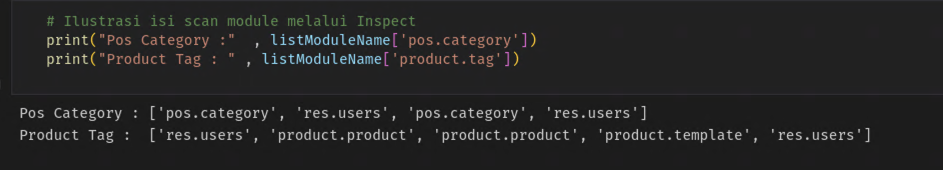
\includegraphics[width=1\textwidth]{img/bab_4/IlustrasiScan.png}
	\caption{Ilustrasi Hubungan antar model Odoo }
	\label{fig:example}
\end{figure}

\subsubsection{Pengabungan dan Optimisasi Hasil Ekstraksi}
Hubungan ketergantungan yang sudah dihasilkan dari PyCG dan inspect, diproses dan dijadikan satu kesatuan sebelum dilakukan proses clustering. Hal yang diproses seperti menghapus node yang tidak terpakai atau diluar dari Odoo seperti keterhubungan dengan library ke-3.  Setiap node pada graph dijadikan satu berdasarkan module/package dengan ini pengelompokan tidak berdasarkan setiap instruksi atau fungsi dari program. 

\begin{figure}[htbp]
	\centering
	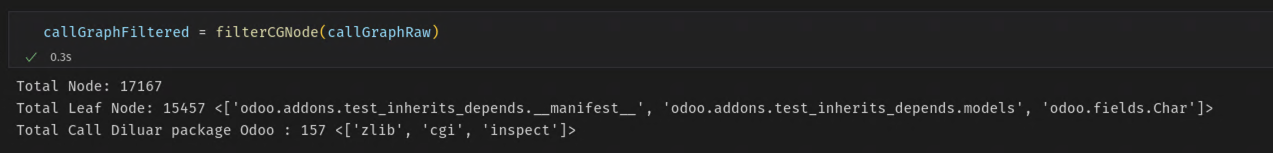
\includegraphics[width=1\textwidth]{img/bab_4/FilterScan.png}
	\caption{Hasil akhir node dari yang sudah digabungkan dan dibersihkan}
	\label{fig:example}
\end{figure}


Jumlah panggilan antara module dijumlahkan untuk dijadikan 'weight' sehingga diketahui module manakah yang paling banyak dipanggil / digunakan. Hasil call graph yang sudah disederhanakan dan difilter maka dapat diubah menjadi matrix adjacency.

\begingroup
\setlength{\LTleft}{-20cm plus -1fill}
\setlength{\LTright}{\LTleft}
\begin{small}
	\begin{longtable}{|p{4cm}|p{3cm}|p{6cm}|}
		\caption{Daftar Metode untuk pengabungan dan optimisasi hasil ekstraksi}\\
		\hline
		\textbf{Metode / Fungsi} & \textbf{Parameter} & \textbf{Keterangan}\\
		\endfirsthead
		
		\hline  

		loadJSON
		& path
		 & Membuka file json dari suatu path  \\

		 \hline  

		 getListRootPackage
		& path
		 & Membuat daftar module/package dari folder path bila folder tersebut memiliki Python. \\

		 \hline  

		 addPrefixFolder
		& cg,root,listPackage
		 & Menambahkan awal root dari call graph yang dihasilkan dari PyCG(JSON) dan disatukan berdasarkan nama modulenya  \\
		 

		 \hline  

		 mergeCGOdooWithAddons
		& cgOdoo,cgAddons
		 & Mengabungkan call graph dari odoo dan addons yang sudah memiliki prefix  \\


		 \hline  

		 filterCGNode
		& cgSource
		 & Menghapus node atau hubungan yang tidak di dalam module addons atau base pada graph \\

		 \hline
		
		 updateCGwInspect
		& listModuleName, moduleNameMapping, callGraph
		 & Mengabungkan hasil relasi yang ditemukan di library inspect ke call graph  \\

		 \hline
		 initKeyCG
		 
			& -
		 & Membuat node untuk graph dari module odoo dan addons kecuali module test dan l10n  \\
		 
		 \hline
		 searchParentCall
		 
			& arrStr
		 & Mencari root atau parent dari sebuah module\\

		 \hline
		
		 updateCGWeight
		& callGraphFiltered, callGraphWeight
		 & Membuat call graph yang memiliki nilai berbobot (weighted graph) berdasarkan jumlah panggilan(call) dengan cara menjumlahkan call yang dipanggil dari module \\

		 
		 \hline
		

		 
		 cleanUpCG
		 
			& callGraph
		 & Menghilangkan call yang rendundan dan  menyimpan informasi panggilan internal di callGraph terpisah\\

		 \hline
		 removeNotConnectedNode
		& callGraph
		 & Menghapus node parent yang tidak terhubung ke node lain \\
		

		 \hline  
		createAdjacentMatrix
		& graphSource
		 & Membuat adjacency matrix dari graph  \\
		
		 \hline  
		 
	\end{longtable}
\end{small}
\endgroup



\subsubsection{Hierarchical Clustering}
Proses ini dilakukan untuk menemukan pengelompokan yang dari adjacency matrix. Matrix adjacency(Matrix keterhubungan) ini harus dihitung kembali nilai kedekatannya, perhitungan tersebut menghasilkan Distance Matrix(Matrik kedekatan). Pada tugas akhir ini menggunakan nilai kedekatan berdasarkan nilai Jaccard dan Struktural Similarity. 

\begin{figure}[htbp]
	\centering
	\includegraphics[width=0.5\textwidth]{img/bab_4/HeatmapModule.png}
	\caption{Heatmap yang menunjukan intensitas hubungan antar module/node}
	\label{fig:heatmap_gambar}
\end{figure}

Matriks kedekatan bisa ditampilan dalam bentuk heatmap. Heatmap dapat memberikan bagaimana intensitas kedekatan antar module addons Odoo. Pada gambar \ref{fig:heatmap_gambar} dapat dilihat semakin kuning atau cerah maka semakin tinggi intensitas hubungannya sedangkan semakin hijau atau redup maka intensitas hubungannya rendah. heatmap ini dihasilkan dari matrix segitiga sehingga hasil dari heatmap sisi kiri sama dengan heatmap sisi kanan.


\begingroup
\setlength{\LTleft}{-20cm plus -1fill}
\setlength{\LTright}{\LTleft}
\begin{small}
	\begin{longtable}{|p{4cm}|p{3cm}|p{6cm}|}
		\caption{Daftar Metode untuk proses Clustering}\\
		\hline
		\textbf{Metode / Fungsi} & \textbf{Parameter} & \textbf{Keterangan}\\
		\endfirsthead
		
		\hline  

		simStr
		& ci, cj, i, j, callsinCi , callsinC
		 & Implementasi dari rumus 2.2  \\

		 \hline  

		 simJaccard
		& im1, im2
		 & Implementasi dari rumus 2.1   \\

		 \hline  

		 calculateDistanceMatrix
		& adjMatrix
		 & Menghitung distance matrix dengan masukan adjacency matrix  \\

		 \hline  

		 visualizeHeatmap
		& matrix, title
		 & Membuat visualisasi heatmap  \\

		 \hline  

		 calculateCluster
		& y, {\_}method
		 & Melakukan proses clustering dengan linkage function tertentu ({\_}method) dan distance matrix (y) \\

		 \hline
		
		 visualizeDendogram
		& z, {\_}method
		 & Menampilakan dendogram dari hierarchical clustering  \\

		 \hline
	\end{longtable}
\end{small}
\endgroup

Distance Matrix dimasukan kedalam fungsi calculateCluster dengan metode ada 3 yaitu average, min, max. Hasil cluster dari hierarchical clustering bisa divisualisasi dalam bentuk dendogram. Hasil dendogram memiliki distance/jarak antar module dan label module. Dari gambar \ref{fig:dd_single} module cenderung dikelompokan dengan jumlah yang kecil (1-2) dan ketika dihubungkan memiliki jarak yang jauh. Pada pendekatan \ref{fig:dd_complete} module dikelompokan dan memiliki ukuran module yang besar untuk setiap partisi/service. Sedangkan pendekatan \ref{fig:dd_avg} memiliki bentuk campuran antara ukuran module yang besar dan module yang berukuran kecil.

\begin{figure}[htbp]
	\centering
	\begin{minipage}{1\textwidth}
		\centering
		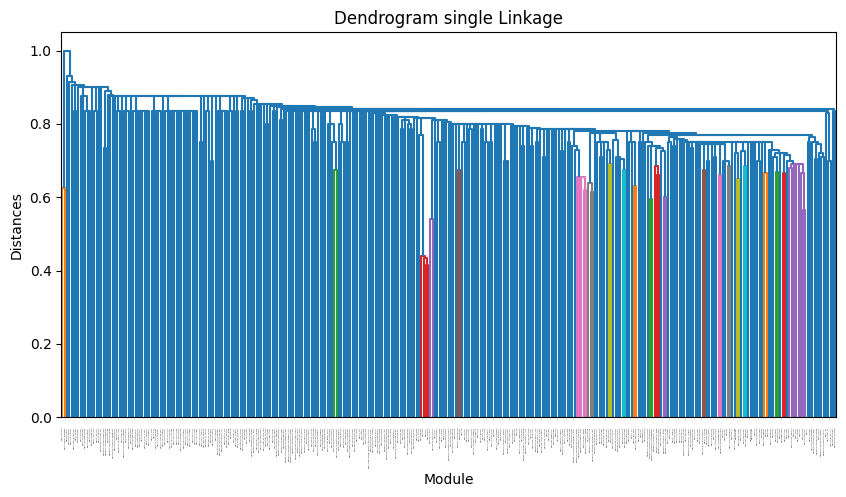
\includegraphics[width=1\textwidth]{img/bab_4/single_dd.png}
		\caption{Dendogram Single Linkage }
		\label{fig:dd_single}
	\end{minipage}\hfill	
\end{figure}

\begin{figure}[htbp]
	\centering
	\begin{minipage}{1\textwidth}
		\centering
		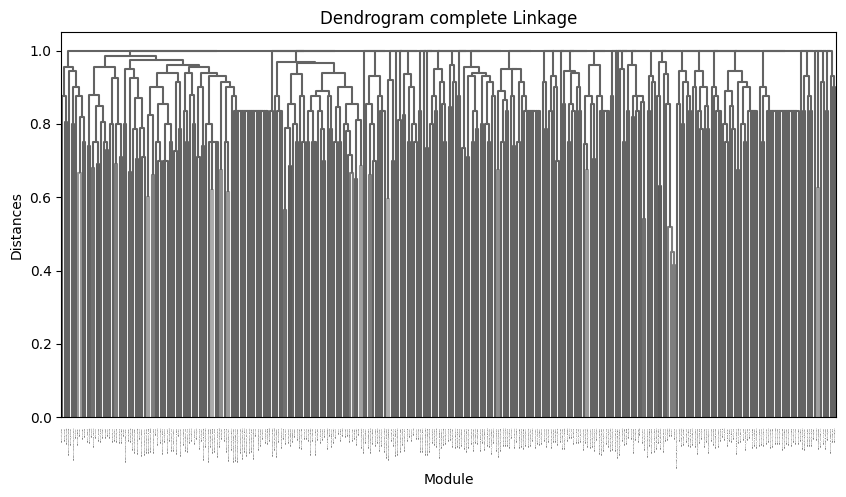
\includegraphics[width=1\textwidth]{img/bab_4/complete_dd.png}
		\caption{Dendogram Complete Linkage }
		\label{fig:dd_complete}
	\end{minipage}\hfill	
\end{figure}

\begin{figure}[htbp]
	\centering
	\begin{minipage}{1\textwidth}
		\centering
		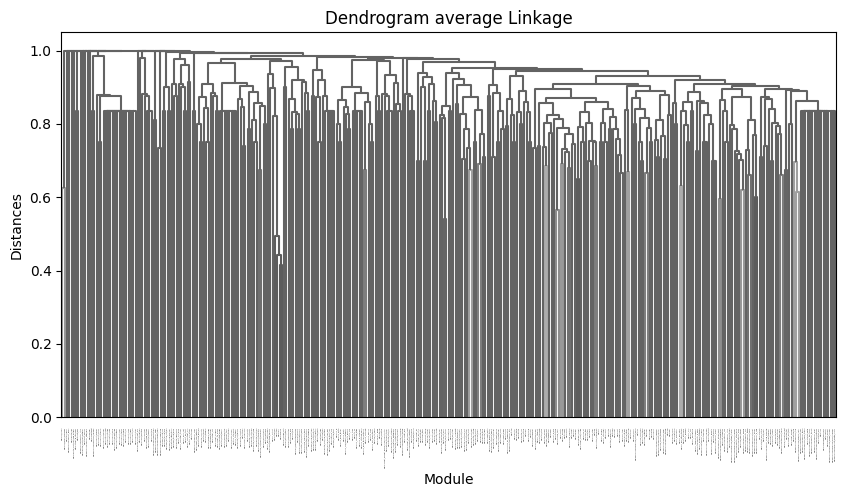
\includegraphics[width=1\textwidth]{img/bab_4/avg_dd.png}
		\caption{Dendogram Average Linkage }
		\label{fig:dd_avg}
	\end{minipage}\hfill	
\end{figure}

\pagebreak

\subsubsection{Pemilihan Partisi}
Banyaknya partisi dan jumlah node, membuat proses pemilihan partisi atau kelompok service terbaik harus dilakukan melalui komputer. Untuk mengetahui jumlah partisi yang tepat dapatdilakukan pengukuran dari nilai coupling dan nilai kohesinya yang dihasilkan dari pengelompokan tersebut. Terdapat fungsi yang akan menghitung dari 1 partisi/service hingga jumlah maximum partisi. 

\begingroup
\setlength{\LTleft}{-20cm plus -1fill}
\setlength{\LTright}{\LTleft}
\begin{small}
	\begin{longtable}{|p{4cm}|p{3cm}|p{6cm}|}
		\caption{Daftar Metode untuk pemilihan Partisi}\\
		\hline
		\textbf{Metode / Fungsi} & \textbf{Parameter} & \textbf{Keterangan}\\
		\endfirsthead
		
		\hline  

		mergeClass
		& ct
		 &  Mencari keterhubungan antar partisi dan di dalam partisi berdasarkan tree yang diberikan dari cluster \\

		 \hline  

		 cutTreeToCluster
		& ct
		 & Membuat cluster dari tree yang dihasilkan clustering  \\

		 \hline  

		 NbCalls
		& m, c1, c2
		 & Menghitung jumlah call antar module (Rumus 2.5) \\

		 \hline  
		 CoupP
		 
		& m, c1,c2
		 & Implementasi dari rumus 2.5   \\

		 \hline  

		 InterCoup
		& m
		 & Implementasi dari rumus 2.4 \\

		 \hline
		
		 InterCoh
		& rm
		 & Implementasi dari rumus 2.6  \\

		 \hline
		 
		 FOne
		& m , rm
		 & Implementasi dari rumus 2.3 dan perhitungan skor clustering melalui jumlah partisi, nilai coupling dan nilai cohesion \\

		 \hline
		 calculateFOne
		& z, {\_}n{\_}clusters
		 & Menghitung hasil FOne dengan diberikan z dan jumlah cluster/partisi \\

		 \hline
		 analystCluster
		& z
		 & Melakukan perhitungan calculateFOne dari 1 hingga jumlah maximum cluster/partisi \\ 


		 \hline
		 visualizeQualityCluster
		& qualityCluster, linkageType
		 & Menampilkan plot perbandingan coupling dan cohesion dengan jumlah service  \\

		 \hline
	\end{longtable}
\end{small}
\endgroup

Hasil pemilihan dapat membantu dalam membuat microservice yang memiliki nilai cohesion yang tinggi dan nilai coupling yang rendah. Pada grafik \ref{fig:cc_avg} dilihat bahwa linkage average memiliki nilai coupling yang rendah, nilai cohesion yang tinggi dan jumlah service yang banyak. Jumlah service yang ideal menurut linkage average yaitu 190-205. 

\begin{figure}[htbp]
	\centering
	\begin{minipage}{1\textwidth}
		\centering
		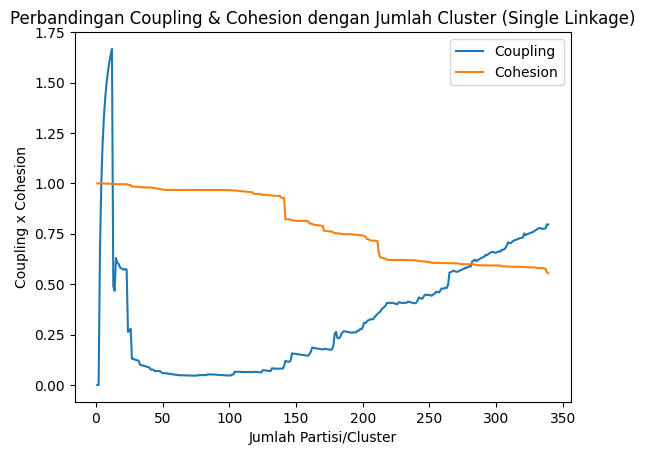
\includegraphics[width=1\textwidth]{img/bab_4/cc_single.png}
		\caption{Pemilihan Partisi terbaik menurut pendekatan Single Linkage }
		\label{fig:cc_single}
	\end{minipage}\hfill	
\end{figure}

\begin{figure}[htbp]
	\centering
	\begin{minipage}{1\textwidth}
		\centering
		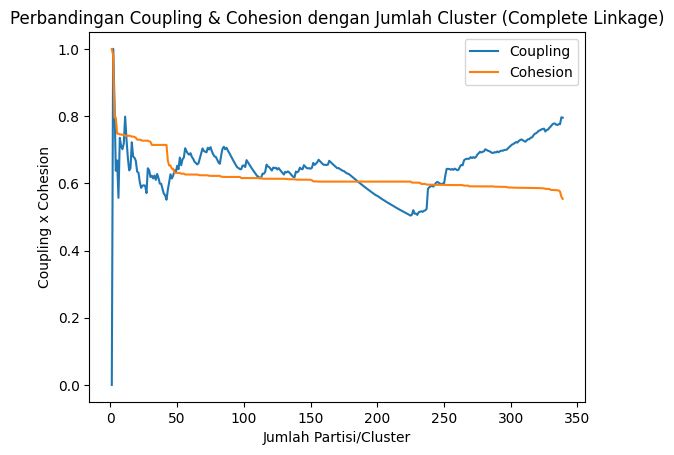
\includegraphics[width=1\textwidth]{img/bab_4/cc_comp.png}
		\caption{Pemilihan Partisi terbaik menurut pendekatan Complete Linkage }
		\label{fig:cc_complete}
	\end{minipage}\hfill	
\end{figure}

\begin{figure}[htbp]
	\centering
	\begin{minipage}{1\textwidth}
		\centering
		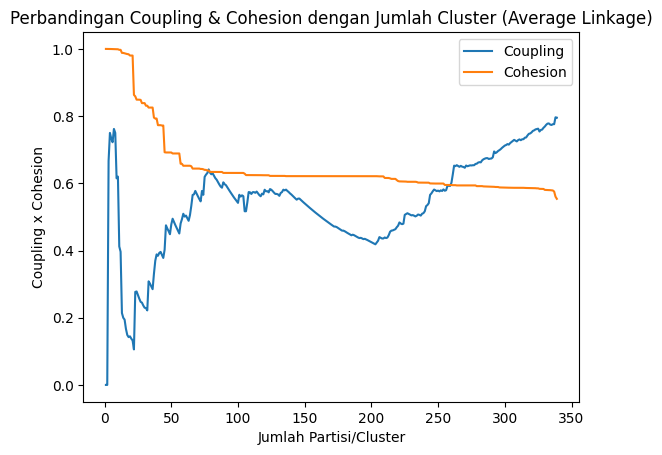
\includegraphics[width=1\textwidth]{img/bab_4/cc_avg.png}
		\caption{Pemilihan Partisi terbaik menurut pendekatan Average Linkage }
		\label{fig:cc_avg}
	\end{minipage}\hfill	
\end{figure}


Pada grafik \ref{fig:cc_single} dilihat linkage single memiliki nilai yang bagus tetapi jumlah service yang ideal hanya sekitar 130-140 service. Sedangkan linkage complete/max (\ref{fig:cc_complete}) memiliki nilai kohesi rendah dan coupling tinggi namun nilai tersebut membaik setelah mencapai kurang lebih 210 jumlah cluster/service.\\


\subsection{Dekomposisi Monolitik \textit{ ke Microservice}}

\subsubsection{\textit{Endpoint API}}
Pada Tabel \ref{tab:endpoint-api} dijelaskan endpoint dan routing yang dipakai dalam masing-masing service. Endpoint tersebut digunakan untuk melakukan uji beban dan pengukuran penggunaan sumber daya dengan sistem monolitik yang sudah dibuat.  

Untuk Client berkomunikasi dengan service maka harus melalui API Gateway dan setiap service untuk mencari service lainnya dapat diarahkan oleh API Gateway. API Gateway membuat rute berdasarkan URL path yang sudah dikonfigurasi sebelumnya serta service dan API Gateway berada di jaringan yang sama.

Berikut IP Address dan port yang digunakan setiap service:
\begin{enumerate}[leftmargin=1.3cm]
	\item Kong Gateway $\rightarrow$ 172.18.0.5:8000
	\item Monolitik $\rightarrow$ 172.18.0.55:8069
	\item Web Service(Frontend) $\rightarrow$ 172.18.0.57:8069
	\item Product Service $\rightarrow$ 172.18.0.51:1323
	\item Point of Sale Service $\rightarrow$ 172.18.0.52:1323
\end{enumerate}

\begingroup
\setlength{\tabcolsep}{6pt} % Adjust the column separation as needed
\begin{small}
	\begin{longtable}{|c|p{3cm}|p{3cm}|p{6cm}|}
	\caption{Tabel Endpoint API} \label{tab:endpoint-api} \\
	\hline
	\textbf{Metode} & \textbf{Route} & \textbf{Body} & \textbf{Keterangan} \\
	\hline
	\endfirsthead
	
	\multicolumn{4}{c}%
	{{\tablename\ \thetable{} -- Lanjutan dari halaman sebelumnya}} \\
	\hline
	\textbf{Metode} & \textbf{Route} & \textbf{Body} & \textbf{Keterangan} \\
	\hline
	\endhead
	
	\hline \multicolumn{4}{|r|}{{Lanjutan di halaman berikutnya}} \\ \hline
	\endfoot
	
	\hline
	\endlastfoot
	
	\multicolumn{4}{|c|}{Monolith (/web/session/*)} \\
	\hline
	POST & /authenticate & JSON, Format: JSON-RPC & Melakukan sesi autentikasi pengguna \\
	\hline
	POST & /destroy & JSON, Format: JSON-RPC & Menghilangkan sesi autentikasi pengguna \\
	\hline
	
	\multicolumn{4}{|c|}{Point of Sales Service (/web/dataset/call\_kw/pos.category/*)} \\
	\hline
	POST & /read & JSON, Format: JSON-RPC & Mendapatkan data Point Of Sale Category \\
	\hline
	POST & /create & JSON, Format: JSON-RPC & Menambahkan data Point Of Sale Category \\
	\hline
	
	\multicolumn{4}{|c|}{Product Service (/web/dataset/call\_kw/product.tag/*)} \\
	\hline
	POST & /read & JSON, Format: JSON-RPC & Mendapatkan data Tag pada product\\
	\hline
	POST & /create & JSON, Format: JSON-RPC & Menambahkan  data Tag pada product \\
	\hline
	
	\multicolumn{4}{|c|}{Web / Frontend Service (/web/*)} \\
	\hline
	GET & /* & - & Mendapatkan data static seperti image, attachment, translation, dan lainnya  \\
	\hline
	
	\end{longtable}
	\end{small}
\endgroup


\subsubsection{ Daftar Class}
Pada bagian ini dijelaskan class yang digunakan PosCategory dan ProductTag :

\begin{longtable}{|c|p{3cm}|p{3cm}|p{4cm}|}
	\caption{Tabel class yang digunakan}
	\label{tab:daftar-class}\\
	\hline
	\textbf{Class} & \textbf{Atribut} & \textbf{Tipe Data} & \textbf{Keterangan} \\
	\hline
	\endfirsthead
	\hline
	\multicolumn{4}{|c|}{\textbf{Dilanjutkan di Halaman Selanjutnya}} \\
	\hline
	\textbf{Class} & \textbf{Atribut} & \textbf{Tipe Data} & \textbf{Keterangan} \\
	\hline
	\endhead
	\hline
	\multicolumn{4}{|c|}{\textbf{Lanjutan Isi Tabel Sebelumnya}} \\
	\hline
	\endfoot
	\hline
	\endlastfoot
	ResUser & UID & int & Class yang menyimpan informasi mengenai pengguna aplikasi/ Odoo. Hampir semua aktivitas pengguna harus dicatat dan harus divalidasi melalui GroupID. Informasi ini dimasukan dari nilai JWT yang disimpan client \\
	\cline{2-3}
	& DisplayName & string & \\
	\cline{2-3}
	& GroupID & int & \\
	\hline
	AccessControlList & GroupID & int & Class yang menyimpan hak akses suatu model atau resource dan dapat dilihat nilai GroupID. Hak akses ini dikomunikasikan dalam waktu tertentu oleh masing-masing service.  \\
	\cline{2-3}
	& ModelID & int & \\
	\cline{2-3}
	& Read & bool & \\
	\cline{2-3}
	& Write & bool & \\
	\cline{2-3}
	& Create & bool & \\
	\cline{2-3}
	& Unlink & bool & \\
	\hline

	\multicolumn{4}{|c|}{\textbf{Point of Sales}} \\
	\hline
	PosCategory & ID & uint & PosCategory atau Point of Sales Category adalah untuk membantu mengelola barang yang yang didagangkan melalui Point of Sale. Kategori ini bisa memiliki tingkatan kategori dan gambar dari kategori tersebut. \\
	\cline{2-3}
	& ParentID & uint & \\
	\cline{2-3}
	& Name & string & \\
	\cline{2-3}
	& Sequence & int & \\
	\cline{2-3}
	& Image &  PosCategoryImage & \\
	\cline{2-3}
	& CreateAt & Timestamp & \\
	\cline{2-3}
	& CreatUID & ResUser & \\
	\cline{2-3}
	& WriteAt & Timestamp & \\
	\cline{2-3}
	& WriteUID & ResUser & \\

	\hline
	PosCategoryImage & UID & int & Merupakan object yang menyimpan informasi gambar yang dimiliki oleh kategori. Gambar disimpan didatabase dan memiliki IdAttachment yang diketahui oleh sistem monolith\\
	\cline{2-3}
	& ImageBase64 & string & \\
	\cline{2-3}
	& AttachmentId & int & \\
	\cline{2-3}
	& ImageSizeByte & int & \\
	\hline

	\multicolumn{4}{|c|}{\textbf{Product}} \\
	\hline
	ProductTag & ID & uint & Product Tag adalah model yang mengelola banyak label untuk memudahkan pencarian disuatu  produk. Product Tag memiliki satu nama yang unik tetapi bisa dimiliki oleh banyak produk template atau produk-produk (varian) \\
	\cline{2-3}
	& Color & uint & \\
	\cline{2-3}
	& Name & string & \\
	\cline{2-3}
	& CreateAt & Timestamp & \\
	\cline{2-3}
	& CreatUID & ResUser & \\
	\cline{2-3}
	& WriteAt & Timestamp & \\
	\cline{2-3}
	& WriteUID & ResUser & \\
	\cline{2-3}
	& ProductTemplate & int[] & \\
	\cline{2-3}
	& ProductProduct & int[] & \\
	\hline
\end{longtable}



\subsubsection{\textit{Docker} }
Pada tugas akhir ini menggunakan teknologi Docker untuk membangun dan mendistribusikan aplikasi dalam bentuk container. Setiap service akan terhubung pada jaringan yang sama. Setiap service termasuk aplikasi monolih memiliki image yang bisa dilakukan deployment antar platform. 

Berikut adalah inisialisasi untuk membuat container dari masing-masing service, setiap serive berada di jaringan internal odoo yang sudah ditentukan sebelum. Tujuannya agar pemetaan service bisa dilukan dengan target ip yang konsisten.

\begin{lstlisting}[style=mystyle, language=sh, caption={Shell Script untuk pembuatan jaringan }]
$ docker network create --subnet=172.18.0.0/16 mono-net
$ docker network create --subnet=172.18.0.0/16 odoo-ms-net	
\end{lstlisting} 

\begin{lstlisting}[style=mystyle, language=sh, caption={Shell Script untuk pembuatan containe microservice }]
$ docker run -d --name odoo-kong-gateway \
	--network=odoo-ms-net \
	--ip 172.18.0.5 \
	-v "$(pwd):/kong/declarative/" \
	-e "KONG_DATABASE=off" \
	-e "KONG_DECLARATIVE_CONFIG=/kong/declarative/kong.yml" \
	-e "KONG_PROXY_ACCESS_LOG=/dev/stdout" \
	-e "KONG_ADMIN_ACCESS_LOG=/dev/stdout" \
	-e "KONG_PROXY_ERROR_LOG=/dev/stderr" \
	-e "KONG_ADMIN_ERROR_LOG=/dev/stderr" \
	-e "KONG_ADMIN_LISTEN=0.0.0.0:8001" \
	-p 8000:8000 \
	-p 8001:8001 \
	-p 8002:8002 \
	-p 8003:8003 \
	kong/kong-gateway:latest 
$ docker run -v "/ubuntu/local":/home/odoo/shared_data --net odoo-ms-net  --ip 172.18.0.55 --name odoo-mono -p :8069  -d odoo-mono
$ docker run -v "/ubuntu/local":/home/odoo/shared_data --net odoo-ms-net  --ip 172.18.0.57 --name odoo-web -p :8069 -d odoo-fe
$ docker run --net odoo-ms-net --ip 172.18.0.54 --name odoo-mariadb -e MYSQL_ROOT_PASSWORD=mariadb -p 3306:3306 -d mariadb 
$ docker run --net odoo-ms-net  --ip 172.18.0.11 --name postgres-odoo -e POSTGRES_PASSWORD=postgres -p 5432:5432 -d postgres
\end{lstlisting} 


\subsubsection{ \textit{Kong}}
Proses selanjutnya yaitu membuat Api Gateway, tugas akhir ini menggunakan Kong sebagai api gateway. Konfigurasi Kong yang digunakan tidak menggunakan database tetapi berupa konfigurasi statik berupa file .yml/.json. Tugas akhir ini menggunakan yml.

Endpoint yang diset adalah keterangan service (ip address,port,protocol) dan routing (metode, apakah host di rewrite ketika dialihkan). Dengan api gateway client hanya perlu mengetahui endpoint pusat kong yaitu :8000. Ketika pencarian rute url tidak ditemukan maka otomatis diarah service monolith (odoo-mono).

\begin{lstlisting}[style=mystyle, language=sh, caption={Konfigurasi Service Monolith }]
- name: odoo-mono
  port: 8069
  protocol: http
  host: 172.18.0.55
  routes:
  - name: odoo-mono-route
    methods:
        - GET
        - POST
        - PUT
        - DELETE
        - PATCH
        - HEAD
        - OPTION
    paths:
    - /
    strip_path: false
    preserve_host: true
\end{lstlisting} 

\begin{lstlisting}[style=mystyle, language=sh, caption={Konfigurasi Service Web/Frontend }]
- name: odoo-web
  port: 8069
  protocol: http
  host: 172.18.0.57
  routes:
  - name: odoo-web-route
    methods:
        - GET
    paths:
    - /web
    strip_path: false
    preserve_host: true
  - name: odoo-web-post-route
    methods:
        - POST
    paths:
    - /web/webclient
    - /web/bundle
    - /web/view
    - /web/content
    - /web/filestore
    - /web/assets
    - /web/action
    - /web/image
    strip_path: false
    preserve_host: true  
\end{lstlisting} 

\begin{lstlisting}[style=mystyle, language=sh, caption={Konfigurasi Service Point of Sale }]
- name: odoo-pos
  port: 1323
  protocol: http
  host: 172.18.0.51
  path: /jsonrpc
  routes:
  - name: odoo-pos-route
    methods:
        - POST
    paths:
    - /web/dataset/call_kw/pos.category/create
    - /web/dataset/call_kw/pos.category/write
    - /web/dataset/call_kw/pos.category/unlink
    - /web/dataset/call_kw/pos.category/read
    strip_path: false
    preserve_host: true
\end{lstlisting} 

\begin{lstlisting}[style=mystyle, language=sh, caption={Konfigurasi Service Product }]
- name: odoo-product
  port: 1323
  protocol: http
  host: 172.18.0.52
  path: /jsonrpc
  routes:
  - name: odoo-product-route
    methods:
        - POST
    paths:
    - /web/dataset/call_kw/product.tag/create
    - /web/dataset/call_kw/product.tag/write
    - /web/dataset/call_kw/product.tag/unlink
    - /web/dataset/call_kw/product.tag/read
    strip_path: false
    preserve_host: true	
\end{lstlisting} 
	

\section{Implementasi Migrasi Arsitektur}
\subsection{Pemisahan User Interface}
Sistem monolith sebelumnya tanggung jawab Frontend dan backend dijadikan satu kesatuan. Permasalah muncul adalah pengaksesan user interface yang jarang berubah bisa menjadi hambatan performa dan skalabilitas. 
Untuk itu setiap permintaan data static sudah ada didalam aplikasi bisa dibagikan tanpa harus menyibukan bagian backend. Untuk menampilkan data odoo membutuhkan informasi yang sama dengan monolith, contohnya ketika mencari file didalam server ,sehingga terdapat dataabase yang dengan monoliht tapi untuk proses yang dapat mengubah data hanya dari monolith.

Di gambar ... dapat dilihat permintaan bisa dibagi ke masing-masing service. 
Ketika kondisi monolith tidak dapat diakses, aplikasi masih bisa dibuka namun dengan fitur yang terbatas.

\subsection{Penerapan JSON Web  Token(JWT)}
Perubahan migrasi arsitektur dari monolith ke microservice, membuat diperlukan sistem pengelolaan hak akses yang stateless. Sehingga service tidak sering harus berkomunikasi satu sama lain terutama pada hal informasi yang sama. Token disimpan didalam cookie client, sehingga baik dari client yang melalui user-interface atau pun secara langsung API, bisa diidentifikasi selama client tersebut memberikan token di cookie ketika meminta data.

\begin{lstlisting}[style=mystyle, language=java, caption={Isi data berupa JSON di JWT}]
{
  "uid": 2,
  "user_context": {
    "lang": "en_US",
    "tz": "Europe/Brussels",
    "uid": 2
  },
  "db": "odoo_db",
  "company_id": 1,
  "partner_id": 3,
  "group_id": [
    2,22,7,34,48
  ],
  "exp": 1692576855
}
\end{lstlisting} 


Untuk menambahkan JWT bisa dituliskan pada proses login sendiri seperti pada \ref{fig:sessionRoute} file py yaitu addons / web/ controlers / session.py . Pada route  /web/session/authenticate 
\begin{figure}[htbp]
	\centering
	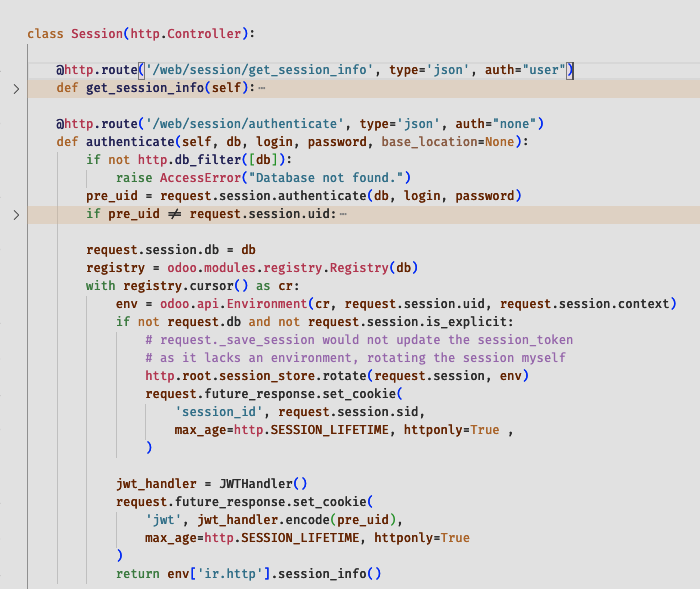
\includegraphics[width=0.7\textwidth]{img/bab_4/sessionRoute.png}
	\caption{Penggalan Kode untuk disisipi proses JWT}
	\label{fig:sessionRoute}
\end{figure}

Data yang disimpan oleh JWT penting diketahui secara umum service, seperti pengguna, konteks pengguna(bahasa, zona waktu), perusahaan, dan database(db).  Perusahaan dan database diperlukan karena odoo memiliki fitur untuk memilih database dan untuk memanggil  aplikasi monolith(Odoo) harus diketahui databasenya. JWT ini dibuat oleh aplikasi monolith ketika login dan dihapus ketika logout atau sesi sudah habis(exp). Masa hidup JWT sama dengan masa hidup session-token yaitu 3 bulan.

Untuk menghancurkan sesi maka ditambahakan mekanisme berupa cookie yang menunjukan bahwa jwt sudah tidak valid. Kemudian cookie tersebut akan dicek oleh fungsi di odoo / http.py / Request.savesession untuk menghapus cookie dengan nama 'jwt' . 
\begin{figure}[htbp]
	\centering
	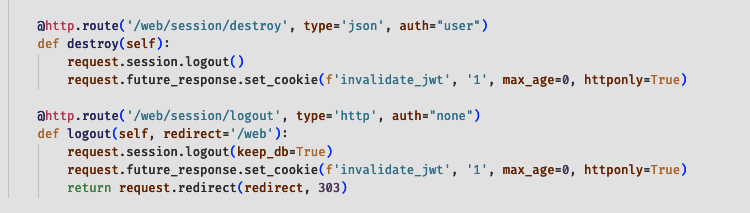
\includegraphics[width=0.8\textwidth]{img/bab_4/triggerCookieDel.png}
	\caption{Potongan Kode untuk memberikan validasi bawah JWT tidak valid}
	\label{fig:example}
\end{figure}

\begin{figure}[htbp]
	\centering
	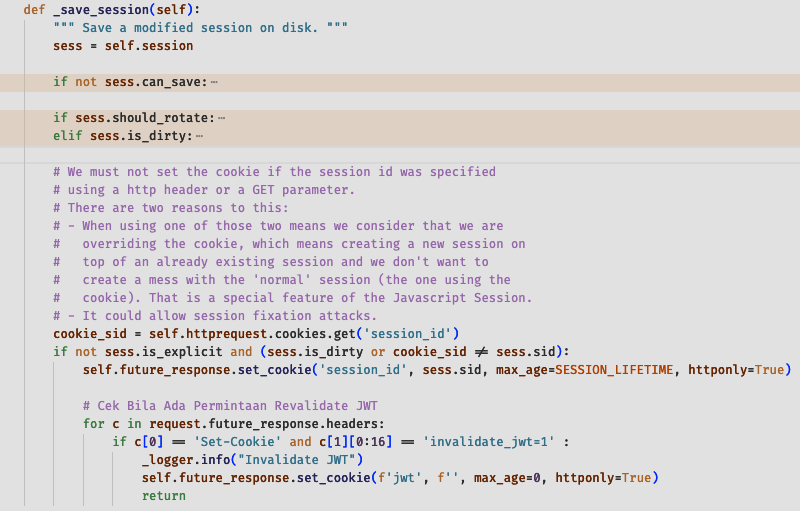
\includegraphics[width=0.8\textwidth]{img/bab_4/removeCookie.png}
	\caption{Potongan Kode untuk memberikan validasi bawah JWT tidak valid}
	\label{fig:example}
\end{figure}



\subsection{Pola Strangle}
Perubahan arsitektur dari aplikasi monolith menjadi microservice membutuhkan banyak resiko dan sumber daya untuk itu perubahan sebaiknya tidak mengurangi atau memperburuk aplikasi yang sudah jadi. Setiap proses bisnis odoo selalu mengimplementasikan class MetaModel. MetaModel membantu pengembang bisa membuat cepat aplikasi tapi MetaModel memiliki keterkaitan dengan model lainnya tinggi. Model di Odoo bisa mengelola data seperti menyimpan di database, memanggil model lainnya, data untuk tampilan(Frontend), dan hal lainnya.

Di MetaModel terdapat fungsi umum dan fungsi internal yang bisa di'override'. Fungsi tersebut dapat dijadikan sebuah adapter. Fungsi utama yang selalu ada pada model yaitu fungsi create, browse, unlink, \_read dan read. Fungsi dan metode tersebut berfungsi untuk mengelola data. Model Adapter dibuat untuk mengabstraksi pengelolaan data sehingga implementasi logic bisa dipindahkan atau dialihkan ke service lainnya dan dikomunikasikan melalui panggilan RPC.  

Adapter yang dibuat juga memiliki kemampuan mengelola datanya karena data yang simpan hanyalah data yang diperlukan oleh sistem lainnya, seperti ID yang digunakan sebagai referensi hubungan antar module. Adapter akan mengelola data secara langsung dari database karena adapter harus berkomunikasi dahulu kepada service yang memiliki tanggung jawab data tersebut.

Ketika ditemukan bahwa data yang berbeda maka dilakukan Update dan didapatkan bila tidak ada, namun ketika data tersebut sebelumnya ada tetapi ketika dicek ditemukan tidak ada. Maka adapter akan mencoba menghapus data tersebut, hal ini akan membuat efek berkelanjutan dengan sistem yang lain. Bila ternyata data tersebut tidak dapat dihapus maka data tersebut hanya bisa didapatkan dan tidak bisa diubah.

Pada pemisahan  model PosCategory, proses penyimpanan data baru dapat memiliki sebuah gambar. Untuk itu ketika ada penyimpana gambar maka gambar disimpan pada database untuk dicatat dan kemudian dikirimkan kepada aplikasi monolith untuk data melalui model ir.attachment di RPC agar gambar bisa diakses melalui web. Setiap model pada Odoo memiliki hak akses kepada grup tertentu. Hak akses bisa diasumsikan jarang berubah untuk karena itu agar service mengetahui apakah seorang user memiliki hak akses. Service memiliki jadwal melaui cron job untuk mengecheck apakah ada akses grup baru.

Service diminta untuk mencatat siapa dan kapan data berubah. Sehingga ada relasi kepada res.user relasi ini hanya memiliki ID, DisplayName, dan GroupID. Informasi ini didapatkan melalui data JWT yang dikirimkan oleh client sebelumnya.



\subsection{\textit{Deployment}}
Deployment dapat dilakukan dengan Virtual Machine yaitu Multipass, dimana virtual machine tersebut memiliki Docker. Pemindahan program/service dilakukan dengan membuat image dari DockerFile, kemudian ketika ingin digunakan bisa diubah menjadi bentuk file(.tar) dan diinstall pada komputer lain.

\begin{lstlisting}[style=mystyle, language=sh, caption={Pembuatan VM untuk Deployment }]
$ multipass launch lts --name odoo-vm  --memory 2G --disk 10G --cpus 2
$ multipass launch lts --name odoo-ms-vm  --memory 2G --disk 10G --cpus 2
\end{lstlisting} 

\section{Pengujian}
\subsection{Perancangan Pengujian}
Pengujian menggunakan JMeter untuk mengetahui latensi dan troughtput serta menggunakan ekstensi perfMon untuk melihat kondisi sumber daya yaitu pengunaan memori dan CPU ketika sedang dilakukan pengujian. 
.....
Tread Group/ User : 5 \\
Loop : 10, 100, 200 ,300 ,500 \\
Target:  /web/dataset/call\_kw/pos.category/create , /web/dataset/call\_kw/pos.category/read \\

\subsection{Uji Beban}

Cu sed numquam inciderint, ei minim altera disputando cum, te nec graeco maiorum convenire.\\
\subsection{Pengunaan Sumber Daya}
Cu sed numquam inciderint, ei minim altera disputando cum, te nec graeco maiorum convenire.\\